% This is the Reed College LaTeX thesis template. Most of the work
% for the document class was done by Sam Noble (SN), as well as this
% template. Later comments etc. by Ben Salzberg (BTS). Additional
% restructuring and APA support by Jess Youngberg (JY).
% Your comments and suggestions are more than welcome; please email
% them to cus@reed.edu
%
% See http://web.reed.edu/cis/help/latex.html for help. There are a
% great bunch of help pages there, with notes on
% getting started, bibtex, etc. Go there and read it if you're not
% already familiar with LaTeX.
%
% Any line that starts with a percent symbol is a comment.
% They won't show up in the document, and are useful for notes
% to yourself and explaining commands.
% Commenting also removes a line from the document;
% very handy for troubleshooting problems. -BTS

% As far as I know, this follows the requirements laid out in
% the 2002-2003 Senior Handbook. Ask a librarian to check the
% document before binding. -SN

%%
%% Preamble
%%
% \documentclass{<something>} must begin each LaTeX document
\documentclass[12pt,twoside]{reedthesis}
% Packages are extensions to the basic LaTeX functions. Whatever you
% want to typeset, there is probably a package out there for it.
% Chemistry (chemtex), screenplays, you name it.
% Check out CTAN to see: http://www.ctan.org/
%%
\usepackage{graphicx,latexsym}
\usepackage{amssymb,amsthm,amsmath}
\usepackage{longtable,booktabs,setspace}
\usepackage{chemarr} %% Useful for one reaction arrow, useless if you're not a chem major
\usepackage[hyphens]{url}
\usepackage{rotating}
\usepackage{natbib}
\usepackage{todonotes}

%% Added for comments
\usepackage{color}
\newcommand{\anna}[1]{{\color{blue}[AR: #1]}}

%% Graphics path
\graphicspath{ {figures/} }

% Comment out the natbib line above and uncomment the following two lines to use the new
% biblatex-chicago style, for Chicago A. Also make some changes at the end where the
% bibliography is included.
%\usepackage{biblatex-chicago}
%\bibliography{thesis}

\newcommand{\argmax}{\arg\!\max}

% \usepackage{times} % other fonts are available like times, bookman, charter, palatino

\title{Winning the Clay Prize in Mathematics feat. Barney Potter}
\author{\#bdawg}
% The month and year that you submit your FINAL draft TO THE LIBRARY (May or December)
\date{May 2016}


%\division{Mathematics and Natural Sciences}
\advisor{Dr. Anna Ritz}
%If you have two advisors for some reason, you can use the following
\altadvisor{Dr. James Fix}
%%% Remember to use the correct department!
\department{Interdisciplinary Committee for Mathematics \& Biology}
% if you're writing a thesis in an interdisciplinary major,
% uncomment the line below and change the text as appropriate.
% check the Senior Handbook if unsure.
\thedivisionof{The Division of Mathematics \& Natural Sciences}
% if you want the approval page to say "Approved for the Committee",
% uncomment the next line
\approvedforthe{Committee}

\setlength{\parskip}{0pt}
%%
%% End Preamble
%%
%% The fun begins:
\begin{document}

  \maketitle
  \frontmatter % this stuff will be roman-numbered
  \pagestyle{empty} % this removes page numbers from the frontmatter

% Acknowledgements (Acceptable American spelling) are optional
% So are Acknowledgments (proper English spelling)
    \chapter*{Acknowledgements}
	I want to thank a few people.

% The preface is optional
% To remove it, comment it out or delete it.
    \chapter*{Preface}
	This is an example of a thesis setup to use the reed thesis document class.

    \tableofcontents
% if you want a list of tables, optional
    \listoftables
% if you want a list of figures, also optional
    \listoffigures

% The abstract is not required if you're writing a creative thesis (but aren't they all?)
% If your abstract is longer than a page, there may be a formatting issue.
    \chapter*{Abstract}
	The preface pretty much says it all.

	\chapter*{Dedication}
	You can have a dedication here if you wish.

  \mainmatter % here the regular arabic numbering starts
  \pagestyle{fancyplain} % turns page numbering back on

%The \introduction command is provided as a convenience.
%if you want special chapter formatting, you'll probably want to avoid using it altogether

    \chapter*{Introduction}
         \addcontentsline{toc}{chapter}{Introduction}
	\chaptermark{Introduction}
	\markboth{Introduction}{Introduction}
	% The three lines above are to make sure that the headers are right, that the intro gets included in the table of contents, and that it doesn't get numbered 1 so that chapter one is 1.

% Double spacing: if you want to double space, or one and a half
% space, uncomment one of the following lines. You can go back to
% single spacing with the \singlespacing command.
% \onehalfspacing
% \doublespacing

\anna{General Comments:
\begin{itemize}
 \item In Git, you might get errors when merging lots of files.  The only files you care about are the .tex, .sty, and .bib files - all other intermediate files can be generated by me.  Keeping the PDF committed might be a good idea if Jim doesn't want to compile it.
 \item Try to turn off every other white page - they make it hard to edit.
 \item In the Introduction, you might want to first discuss what cell signaling \textit{is}, biologically.  Perhaps use a case study (e.g., Hedgehog signaling).
 \item Start making your bib file - there are lots of pieces you have written that will need to be cited.
\end{itemize}}

	Cell function is governed by countless interactions between proteins, nucleic acids, lipids, carbohydrates, and many other small molecules.  The interactions between all of these components form what we call \textit{cell signaling networks}, which are responsible for almost every process within a cell.  Cell signaling networks are used to describe how many of the most basic reactions within cells interact with each other.  Some of the most important types of interactions that we see in cell signaling networks include the assembly and destruction of protein complexes, how small molecules such as ATP interact with proteins, the cascade of events that can occur after a membrane-bound protein is bound by a ligand, or where negative feedback loops exist that can have an effect on cell function.  We often refer to these cell signaling networks at protein-protein interaction (PPI) networks.  Historically, PPI networks have been a useful tool for compiling knowledge about individual interactions that have been studied \textit{in situ}, so that larger scale patterns of interaction can be examined, and both communicated easily and   In recent years, there has been a push to find ways to accurately model these networks so that they can be used to predict potential areas of future research (CITATION).


 \section{Representations of PPI Networks}


 \section{Graph Theory}

\chapter{Protein-Protein Interaction Networks}

Since the discovery of cells by Robert Hooke in 1665, biologists have worked tirelessly to unlock the mysteries of cell function. Over the last half-century, our knowledge of how cells function has grown tremendously.

\chapter{Notes, Comments, \& Changelog}

 \anna{What will Chapter 1 be? I am trying to figure out where the biological signaling pathway discussion will be.}

\chapter{Hypergraphs \& Hyperpaths}

 \anna{Sounds like you are discussing limitations of graphs; this can be a separate section ``Limitations of Graphs'' before you mention hypergraphs.}

While standard graphs are useful for many applications, they are severely limited in their ability to represent cell-signaling interactions.  Since they can only show pairwise interactions between nodes, whenever there is an interaction that requires more than two connections, the visualization of the graph becomes confusing, and biologically meaningless.  Furthermore, interactions involving multiple molecules require an enormous amount of different edges to represent all of the sub-interactions that take place.  Determining whether two edges are part of the same biological event is a non-trivial problem, and requires manual curation to solve, at this time.

\textit{Give an example of a specific PPI that would be terrible with standard graphs, but easier with a hypergraph in paragraph below}

One area of cell-signaling that becomes particularly problematic in standard graphs is the formation, interaction, and destruction of protein complexes.  The only way that complexes can be represented in standard graphs is by creating a complete subgraph of all of the elements of the protein complex.  On their own, these complete subgraphs can yield useful information about the make-up of a protein complex, but once they begin interacting with other elements of the graph, the graph becomes much more complex, as all of the proteins in the complex must be represented independently.  In the case of interactions between multiple large complexes, it becomes the case that the standard graph representation of this interaction is a large complete subgraph that contains nodes for all of the proteins involved in either complex.  It is then computationally impossible to distinguish whether the entity being described by the subgraph is the interaction between multiple protein complexes, or simply one large complex that contains all of the components of both complexes.  Furthermore, since the complete subgraphs which represent complexes are undirected, it is not possible \textit{(is this the case?)} to tell what the inputs or outputs of a biochemical reaction may be.

Another shortcoming of standard graphs\footnote{The term ``standard" is used to describe traditional graphs, since the terms ``regular" and ``normal," which would be natural choices, both refer to specific types of graphs.} in representing complex biological interactions is that there is no way in which to represent positive or negative regulation of interactions.  Since there is a standardized way in which edges interact with nodes, there is no way to differentiate types of interactions between nodes.  This poses a challenge when there are regulators or catalysts present that are necessary for a reaction, but are not part of the inputs or outputs of the reaction.  If regulators are to be included in a standard graph representation of a cell-signaling network, they become indistinguishable from any other types of interactions that are taking place.  This lack of specificity is problematic, as it treats all interactions as equal, and hides potentially useful information from the graph.

To resolve the issues presented by standard graphs, we instead use a generalization called a \textit{hypergraph} that allows for the addition of more detail  and specificity within the data structure than standard graphs allow for.  In particular, hypergraphs allow for both the representation of protein complexes in the form of \textit{hypernodes}, which we think of simply as a set of one or more nodes, and for the representation of complex, directed interactions that can have multiple inputs and outputs.  We represent these interactions with the use of \textit{hyperedges}, which define a set of one or more hypernodes.  Since a hyperedge may include more than two hypernodes, we gain the ability to represent both multi-protein interactions, as well as to define the notions of regulation on reactions.

\section{Hypergraph Definitions}

\anna{When discussing hypergraphs, you will need to be clear about when you are citing someone's definition of hypergraphs, or whether you are defining your own terms. }

Where a directed graph represents directed, pairwise interactions between only two vertices, we can use \textit{directed hypergraph} to represent directed interactions between sets of vertices (nodes). We formally define a directed hypergraph, $\mathcal{H}$, as a pair $(V,E)$, where $V$ is a finite set of vertices and $E \subseteq 2^V \times 2^V$ is a finite set of \textit{directed hyperedges} connecting members of $V$ such that, for every $e=(T(e),H(e)) \in E$, $T(e) \cap H(e) = \emptyset$, and $T(e)$, $H(e) \neq \emptyset$.  We refer to $T(e)$ as the \textit{tail} of the hyperedge, and to $H(e)$ as the \textit{head} of the hyperedge.

Furthermore, we can define sets of two or more nodes as a hypernode, which are members of the power set of $V$.  These can be incorporated into a directed hypergraph to form a \textit{complexed directed hypergraph}.  We define a \textit{complexed directed hypergraph}, $\mathcal{H}$, as the triple $(V,U,E)$ in which $V$ is a finite set of vertices, $U \subseteq 2^V$ is a finite set of hypernodes, and $E \subseteq 2^U \times 2^U$ is a finite set of hyperedges such that, for every $e=(T(e),H(e)) \in E$, $T(e) \cap H(e) = \emptyset$ and $T(e)$, $H(e) \neq \emptyset$.

\begin{figure}
  \begin{center}
    \includegraphics{example-hypergraph}
  \caption{An example of a hypergraph where (MAKE NEW FIGURE WHERE NODES AND HPEREDGES ARE LABELED)}
  \end{center}
\end{figure}

It is important to note that a standard directed graph is a special case of a directed hypergraph.  This is the case if every hypernode in the graph contains only one element, and if each edge has exactly one head element, and one tail element.  This has two important implications for algorithms that run on directed hypergraphs.  First, this means that there is no loss in functionality caused by using a hypergraph representation of a cell network, since anything that could be computed on a standard directed graph can be recreated exactly using the special case of the hypergraph. Secondly, this is important, because it means that anything that can be computed on a standard graph will be at least as computationally difficult to compute when generalized to a hypergraph.  In fact, we find that many tasks that are computationally easy on standard graphs become very difficult when generalized to hypergraphs \textit{(cite Anna's paper on K shortest hyperpaths)}.

\section{Hyperpaths \& Connectivity}
In order to find the shortest route between two vertices, in a directed hypergraph, we define the notion of a \textit{hyperpath}, $P$, on the directed hypergraph $\mathcal{H}$.  We think of $P$ as the list of vertices and hyperedges that one must pass through in order to traverse through the directed hypergraph from vertex $u$ to get to $v$. The existence of a hyperpath between two nodes encodes the notion of ``connectivity" between those nodes.  If a hyperpath exists between nodes $u$ and $v$, we say that they are \textit{connected}. Furthermore, we refer to the set of all nodes in a hypergraph that are connected to each other by some hyperpath as a \textit{connected subnetwork} of the hypergraph. This is a useful definition, because it allows us the notion of a \textit{connected hypergraph}, a hypergraph in which every node is connected by some hyperpath to every other node in the hypergraph.

\anna{How does defining hyperpaths contribute to your ``story'' for Steiner Hypertrees?  You might not need to go into a ton of detail here, you really want to use it to motivate Steiner hypertrees.}

\subsection{Definition}

\subsection{Finding \textit{k}-Shortest Hyperpaths}

\section{Algorithms on Hypergraphs}

\subsection{Integer Linear Programming}

\subsection{NP-Hardness}

	\chapter{The Prize-Collecting Steiner Problem}

	\anna{Motivate this by the biological application.  Why do we want to try to do this instead of computing paths?  What does this gain us?}

\section{Prize-Collecting Steiner Trees}

\subsection{Prize-Collecting Steiner Forests}


\chapter{PCST in Directed Signaling Hypergraphs}

\section{PCSHT(Define) Formulation}

\anna{Seems like you haven't committed an ``annotated'' version yet.  Some high-level comments:
\begin{itemize}
\item Spend a couple paragraphs describing the goal of the problem and the optimization.
\item Be sure to list, for each constraint, what the variables range over (``for each hyperedge'' or ``for each node'').
\item Which variables/constants are binary? Which ones are real-valued?
\end{itemize}
}

In order for us define and develop a Prize-Collecting Steiner Hyptertree, we begin by formulating the notion of a \textit{Steiner Hypertree}.  To make our Steiner Hypertree, $\mathcal{S}$, we begin with a ``parent" hypergraph, $\mathcal{H} = (V,E)$, and a set of target nodes, such that $T \subseteq V$.  We refer to each hypernode as some $x$ such that $x \in V$\footnote{We use ``$x$" as an element of $V$, rather than lowercase ``$v$" to avoid the visual confusion between lowercase $v$ and uppercase $V$ (REMOVE THIS IF CHANGING TO V'S LOOKS OKAY)}, and each edge is some $e$ such that $e \in E$.  When building $\mathcal{H}$, we initially seed the hypergraph.  Each hyperedge is assigned a weight, that is, a cost associated with including that edge in $\mathcal{S}$.  We then assign each hypernode in $\mathcal{H}$ two values, a prize for being included in $\mathcal{S}$, as well as a penalty associated with being a \textit{dangling} hypernode.  We say a hypernode is dangling if it is included in $\mathcal{S}$, and it has no incoming hyperedge which is also included in $\mathcal{S}$ (i.e. the vertex is not in the head of any edge in $\mathcal{S}$).\\

We now can define the Steiner Hypertree, $\mathcal{S}$, to be the set of hypernodes and hyperedges for which total vertex prizes are maximized, and total edge weights (and dangling penalties) are minimized.  The Steiner Hypertree produced should satisfy the following properties:

% \begin{itemize}
% 	\item The prizes for vertices included in $\mathcal{S}$ should be maximized.
% 	\item The costs for edges included in $\mathcal{S}$ should be minimized.
% 	\item All members of $T$ are included in $\mathcal{S}$.
% 	\item Each vertex that is incident (included in either the head or the tail) on an edge included in $\mathcal{S}$ is also in $\mathcal{S}$.
% 	\item All vertices included in $\mathcal{S}$ satisfy one of two conditions:
% 	\begin{itemize}
% 		\item The vertex has at least one incoming hyperedge that is also in $\mathcal{S}$.
% 		\item The vertex is dangling.
% 	\end{itemize}
% 	\item Hanging penalties for dangling nodes included in $\mathcal{S}$ are minimized.
% \end{itemize}

	\begin{figure}[h]
		  \centering
		\missingfigure[figwidth=15cm]{Colored example of a parent hypergraph with an example Steiner Hypertree within}
		\caption{Here is an example parent graph, $\mathcal{H}$, and its corresponding Steiner Hypergraph, $\mathcal{S}$.  Target hypernodes, $T$ are shown in red, Steiner hypernodes and hyperedges included in $\mathcal{S}$ are shown in blue, and the the dangling node(s) are in green.}
		\label{fig:shypertree}
	\end{figure}

\section{Steiner Hypertree ILP}

Given an input hypergraph $\mathcal{H}=(V,E)$, and a set of target nodes, $T$, we construct a Steiner Hypertree, (DEFINE) $\mathcal{S}= (V^\prime,E^\prime)$, where $V^\prime \subseteq V$ and $E^\prime \subseteq E$.  We build $\mathcal{S}$ using an ILP which encodes the definition of a Steiner Hypertree.  In order to accomplish this, we define three indicator variables, $\alpha_v$, $\alpha_e$, and $\delta_v$, where $v$ and $e$ are hypernodes or hyperedges in $\mathcal{H}$.  If hypernode $x$ is in the solution of the ILP, $\alpha_v$ will have a value of 1, otherwise it will be equal to 0.  Similarly, if edge $e$ is present in the solution, $\alpha_e$ will take a value of 1. The value of $\delta_v$ will be determined by whether a hypernode is dangling, as described above (DESCRIBE ABOVE).\\

We find the Steiner Hypergraph $\mathcal{S}$ by optimizing the function:

\begin{equation} \label{eq:ilpsum}
 \argmax_{\alpha , \delta} \sum_{v \in V} g_v \alpha_v - \sum_{e \in E} c_e \alpha_e - \sum_{v \in V} h_v \delta_v
\end{equation}

Subject to the set of linear constraints:

\begin{align}
        \alpha_v \geq 1 \qquad\qquad &\forall\; v \in T\label{eq:ilpT}\\
        \sum_{v \in H_e} \alpha_v \geq \lvert H_e\rvert \alpha_e \qquad\qquad &\forall\; v \in H_V , e \in H_E\label{eq:ilpinchead}\\
        \sum_{v \in T_e} \alpha_v \geq \lvert T_e\rvert \alpha_e\qquad\qquad &\forall\; v \in H_V , e \in H_E\label{eq:ilpinctail}\\
        \delta_v \leq \alpha_v \qquad\qquad &\forall\; v \in \mathcal{H}\label{eq:ilpdang1}\\
        \delta_v \geq \alpha_{v} - \sum_{e:v \in H_e} \alpha_e \qquad\qquad &\forall\; v \in \mathcal{H}\label{eq:ilpdang2}\\
        0 \leq \delta_v \leq 1 \qquad\qquad &\forall\; v \in \mathcal{H}\label{eq:ilpdang3}%
\end{align}%


Constraint \eqref{eq:ilpT} encodes that every target node in $T$ is in the solution, $\mathcal{S}$.  Constraints \eqref{eq:ilpinchead} and \eqref{eq:ilpinctail} ensure that if an edge is in $\mathcal{S}$, any nodes incident on that edge will also be in $\mathcal{S}$.  Finally, constraints \eqref{eq:ilpdang1}, \eqref{eq:ilpdang2}, and \eqref{eq:ilpdang3} encode the ability for nodes to dangle if they do not have an incoming edge.  Though this formulation encodes all of the properties of a Steiner Hypertree, on some hypergraphs, it can yield subtrees that are trivial, due to the possibility of simple cycles between target nodes and Steiner nodes.  We solve this problem by introducing one more variable to the program to impose a topological ordering on the nodes.


\chapter{Benchmarking (\& Proof??)}

To assess the efficacy of this ILP in generating the correct Prize Collecting Steiner Hypertree, it is first necessary to perform a series of benchmarking tests on known datasets and hypergraphs.  This will allow us to determine if the algorithm is performing as expected, and generating results that can be corroborated manually.

\chapter{Application to PPI Data}

\chapter{}
%\section{References, Labels, Custom Commands and Footnotes}
%It is easy to refer to anything within your document using the \texttt{label} and \texttt{ref} tags.  Labels must be unique and shouldn't use any odd characters; generally sticking to letters and numbers (no spaces) should be fine. Put the label on whatever you want to refer to, and put the reference where you want the reference. \LaTeX\ will keep track of the chapter, section, and figure or table numbers for you.
%
%\subsection{References and Labels}
%Sometimes you'd like to refer to a table or figure, e.g. you can see in Figure \ref{subd2} that you can rotate figures . Start by labeling your figure or table with the label command (\verb=\label{labelvariable}=) below the caption (see the chapter on graphics and tables for examples). Then when you would like to refer to the table or figure, use the ref command (\verb=\ref{labelvariable}=). Make sure your label variables are unique; you can't have two elements named ``default." Also, since the reference command only puts the figure or table number, you will have to put  ``Table" or ``Figure" as appropriate, as seen in the following examples:
%
% As I showed in Table \ref{inheritance} many factors can be assumed to follow from inheritance. Also see the Figure \ref{subd} for an illustration.
%
%\subsection{Custom Commands}\label{commands}
%Are you sick of writing the same complex equation or phrase over and over?
%
%The custom commands should be placed in the preamble, or at least prior to the first usage of the command. The structure of the \verb=\newcommand= consists of the name of the new command in curly braces, the number of arguments to be made in square brackets and then, inside a new set of curly braces, the command(s) that make up the new command. The whole thing is sandwiched inside a larger set of curly braces.
%
%% Note: you cannot use numbers in your commands!
%\newcommand{\hydro}{H$_2$SO$_4$}
%
%In other words, if you want to make a shorthand for H$_2$SO$_4$, which doesn't include an argument, you would write: \verb=\newcommand{\hydro}{H$_2$SO$_4$}= and then when you needed  to use the command you would type \verb=\hydro=. (sans verb and the equals sign brackets, if you're looking at the .tex version). For example: \hydro
%
%\subsection{Footnotes and Endnotes}
%	You might want to footnote something.\footnote{footnote text} Be sure to leave no spaces between the word immediately preceding the footnote command and the command itself. The footnote will be in a smaller font and placed appropriately. Endnotes work in much the same way. More information can be found about both on the CUS site.
%
%\section{Bibliographies}
%	Of course you will need to cite things, and you will probably accumulate an armful of sources. This is why BibTeX was created. For more information about BibTeX and bibliographies, see our CUS site (\url{web.reed.edu/cis/help/latex/index.html})\footnote{\cite{reedweb:2007}}. There are three pages on this topic: {\it bibtex} (which talks about using BibTeX, at \url{/latex/bibtex.html}), {\it bibtexstyles} (about how to find and use the bibliography style that best suits your needs, at \url{/latex/bibtexstyles.html}) and {\it bibman} (which covers how to make and maintain a bibliography by hand, without BibTeX, at at \url{/latex/bibman.html}). The last page will not be useful unless you have only a few sources. There used to be APA stuff here, but we don't need it since I've fixed this with my apa-good natbib style file.
%
%\subsection{Tips for Bibliographies}
%\begin{enumerate}
%\item Like with thesis formatting, the sooner you start compiling your bibliography for something as large as thesis, the better. Typing in source after source is mind-numbing enough; do you really want to do it for hours on end in late April? Think of it as procrastination.
%\item The cite key (a citation's label) needs to be unique from the other entries.
%\item When you have more than one author or editor, you need to separate each author's name by the word ``and'' e.g.\\ \verb+Author = {Noble, Sam and Youngberg, Jessica},+.
%\item Bibliographies made using BibTeX (whether manually or using a manager) accept LaTeX markup, so you can italicize and add symbols as necessary.
%\item To force capitalization in an article title or where all lowercase is generally used, bracket the capital letter in curly braces.
%\item You can add a Reed Thesis citation\footnote{\cite{noble:2002}} option. The best way to do this is to use the phdthesis type of citation, and use the optional ``type'' field to enter ``Reed thesis'' or ``Undergraduate thesis''. Here's a test of Chicago, showing the second cite in a row\footnote{\cite{noble:2002}} being different. Also the second time not in a row\footnote{\cite{reedweb:2007}} should be different. Of course in other styles they'll all look the same.
%\end{enumerate}
%\section{Anything else?}
%If you'd like to see examples of other things in this template, please contact CUS (email cus@reed.edu) with your suggestions. We love to see people using \LaTeX\ for their theses, and are happy to help.
%
%
%\chapter{Mathematics and Science}
%\section{Math}
%	\TeX\ is the best way to typeset mathematics. Donald Knuth designed \TeX\ when he got frustrated at how long it was taking the typesetters to finish his book, which contained a lot of mathematics.
%
%	If you are doing a thesis that will involve lots of math, you will want to read the following section which has been commented out. If you're not going to use math, skip over this next big red section. (It's red in the .tex file but does not show up in the .pdf.)
%%
%%% MATH and PHYSICS majors: Uncomment the following section
%%
%$$\sum_{j=1}^n (\delta\theta_j)^2 \leq {{\beta_i^2}\over{\delta_i^2 + \rho_i^2}}
%\left[ 2\rho_i^2 + {\delta_i^2\beta_i^2\over{\delta_i^2 + \rho_i^2}} \right] \equiv \omega_i^2
%$$
%
%From Informational Dynamics, we have the following (Dave Braden):
%
%After {\it n} such encounters the posterior density for $\theta$ is
%
%$$
%\pi(\theta|X_1< y_1,\dots,X_n<y_n) \varpropto \pi(\theta) \prod_{i=1}^n\int_{-\infty}^{y_i}
%   \exp\left(-{(x-\theta)^2\over{2\sigma^2}}\right)\ dx
%$$
%
%
%
%Another equation:
%
%$$\det\left|\,\begin{matrix}%
%c_0&c_1\hfill&c_2\hfill&\ldots&c_n\hfill\cr
%c_1&c_2\hfill&c_3\hfill&\ldots&c_{n+1}\hfill\cr
%c_2&c_3\hfill&c_4\hfill&\ldots&c_{n+2}\hfill\cr
%\,\vdots\hfill&\,\vdots\hfill&
%  \,\vdots\hfill&&\,\vdots\hfill\cr
%c_n&c_{n+1}\hfill&c_{n+2}\hfill&\ldots&c_{2n}\hfill\cr
%\end{matrix}\right|>0$$
%
%%
%Lapidus and Pindar, Numerical Solution of Partial Differential Equations in Science and
%Engineering.  Page 54
%
%$$
%\int_t\left\{\sum_{j=1}^3 T_j \left({d\phi_j\over dt}+k\phi_j\right)-kT_e\right\}w_i(t)\ dt=0,
%   \qquad\quad i=1,2,3.
%$$
%
%L\&P  Galerkin method weighting functions.  Page 55
%
%$$
%\sum_{j=1}^3 T_j\int_0^1\left\{{d\phi_j\over dt} + k\phi_j\right\} \phi_i\ dt
%   = \int_{0}^1k\,T_e\phi_idt, \qquad i=1,2,3 $$
%
%Another L\&P (p145)
%
%$$
%\int_{-1}^1\!\int_{-1}^1\!\int_{-1}^1 f\big(\xi,\eta,\zeta\big)
%   = \sum_{k=1}^n\sum_{j=1}^n\sum_{i=1}^n w_i w_j w_k f\big( \xi,\eta,\zeta\big).
%$$
%
%Another L\&P (p126)
%
%$$
%\int_{A_e} (\,\cdot\,) dx dy = \int_{-1}^1\!\int_{-1}^1 (\,\cdot\,) \det[J] d\xi d\eta.
%$$
%
%
%\section{Physics}
%
%Many of the symbols you will need can be found on the math page (\url{http://web.reed.edu/cis/help/latex/math.html}) and the Comprehensive \LaTeX\ Symbol Guide (enclosed in this template download).  You may wish to create custom commands for commonly used symbols, phrases or equations, as described in Chapter \ref{commands}.
%
%\section{Biology}
%You will probably find the resources at \url{http://www.lecb.ncifcrf.gov/~toms/latex.html} helpful, particularly the links to bsts for various journals. You may also be interested in TeXShade for nucleotide typesetting (\url{http://homepages.uni-tuebingen.de/beitz/txe.html}).  Be sure to read the proceeding chapter on graphics and tables, and remember that the thesis template has versions of Ecology and Science bsts which support webpage citation formats.
%
%\chapter{Tables and Graphics}
%
%\section{Tables}
%	The following section contains examples of tables, most of which have been commented out for brevity. (They will show up in the .tex document in red, but not at all in the .pdf). For more help in constructing a table (or anything else in this document), please see the LaTeX pages on the CUS site.
%
%\begin{table}[htbp] % begins the table floating environment. This enables LaTeX to fit the table where it works best and lets you add a caption.
%\caption[Basic Table 1]{A Basic Table: Correlation of Factors between Parents and Child, Showing Inheritance}
%% The words in square brackets of the caption command end up in the Table of Tables. The words in curly braces are the caption directly over the table.
%\begin{center}
%% makes the table centered
%\begin{tabular}{c c c c}
%% the tabular environment is used to make the table itself. The {c c c c} specify that the table will have four columns and they will all be center-aligned. You can make the cell contents left aligned by replacing the Cs with Ls or right aligned by using Rs instead. Add more letters for more columns, and pipes (the vertical line above the backslash) for vertical lines. Another useful type of column is the p{width} column, which forces text to wrap within whatever width you specify e.g. p{1in}. Text will wrap badly in narrow columns though, so beware.
%\toprule % a horizontal line, slightly thicker than \hline, depends on the booktabs package
%  Factors &  Correlation between Parents \& Child & Inherited \\ % the first row of the table. Separate columns with ampersands and end the line with two backslashes. An environment begun in one cell will not carry over to adjacent rows.
%  \midrule % another horizontal line
%Education & -0.49 & Yes \\ % another row
%Socio-Economic Status & 0.28 & Slight \\
%Income & 0.08 & No\\
%Family Size & 0.19 & Slight \\
%Occupational Prestige &0.21 & Slight \\
%\bottomrule % yet another horizontal line
%\end{tabular}
%\end{center}
%\label{inheritance} % labels are useful when you have more than one table or figure in your document. See our online documentation for more on this.
%\end{table}
%
%	\clearpage
%%% \clearpage ends the page, and also dumps out all floats.
%%% Floats are things like tables and figures.
%
%If you want to make a table that is longer than a page, you will want to use the longtable environment. Uncomment the table below to see an example, or see our online documentation.
%
%	\begin{longtable}{||c|c|c|c||}
%	 	\caption[Long Table]{An example of a long table, with headers that repeat on each subsequent page: Results from the summers of 1998 and 1999 work at Reed College done
%by Grace Brannigan, Robert Holiday and Lien Ngo in 1998 and Kate Brown and
%Christina Inman in 1999.}\\ \hline
%	    	  \multicolumn{4}{||c||}{Chromium Hexacarbonyl} \\\hline
%		   State & Laser wavelength & Buffer gas & Ratio of $\frac{\textrm{Intensity
%at vapor pressure}}{\textrm{Intensity at 240 Torr}}$ \\ \hline
%		  \endfirsthead
%		\hline     State & Laser wavelength & Buffer gas & Ratio of
%$\frac{\textrm{Intensity at vapor pressure}}{\textrm{Intensity at 240 Torr}}$\\
%\hline
%		    \endhead
%
%	    $z^{7}P^{\circ}_{4}$ & 266 nm & Argon & 1.5 \\\hline
%	    $z^{7}P^{\circ}_{2}$ & 355 nm & Argon & 0.57 \\\hline
%	    $y^{7}P^{\circ}_{3}$ & 266 nm & Argon & 1 \\\hline
%	    $y^{7}P^{\circ}_{3}$ & 355 nm & Argon & 0.14 \\\hline
%	    $y^{7}P^{\circ}_{2}$ & 355 nm & Argon & 0.14 \\\hline
%	    $z^{5}P^{\circ}_{3}$ & 266 nm & Argon & 1.2 \\\hline
%	    $z^{5}P^{\circ}_{3}$ & 355 nm & Argon & 0.04 \\\hline
%	    $z^{5}P^{\circ}_{3}$ & 355 nm & Helium & 0.02 \\\hline
%	    $z^{5}P^{\circ}_{2}$ & 355 nm & Argon & 0.07 \\\hline
%	    $z^{5}P^{\circ}_{1}$ & 355 nm & Argon & 0.05 \\\hline
%	    $y^{5}P^{\circ}_{3}$ & 355 nm & Argon & 0.05, 0.4 \\\hline
%	    $y^{5}P^{\circ}_{3}$ & 355 nm & Helium & 0.25 \\\hline
%	    $z^{5}F^{\circ}_{4}$ & 266 nm & Argon & 1.4 \\\hline
%	    $z^{5}F^{\circ}_{4}$ & 355 nm & Argon & 0.29 \\\hline
%	    $z^{5}F^{\circ}_{4}$ & 355 nm & Helium & 1.02 \\\hline
%	    $z^{5}D^{\circ}_{4}$ & 355 nm & Argon & 0.3 \\\hline
%	    $z^{5}D^{\circ}_{4}$ & 355 nm & Helium & 0.65 \\\hline
%	    $y^{5}H^{\circ}_{7}$ & 266 nm & Argon & 0.17 \\\hline
%	    $y^{5}H^{\circ}_{7}$ & 355 nm & Argon & 0.13 \\\hline
%	    $y^{5}H^{\circ}_{7}$ & 355 nm & Helium & 0.11 \\\hline
%	    $a^{5}D_{3}$ & 266 nm & Argon & 0.71 \\\hline
%	    $a^{5}D_{2}$ & 266 nm & Argon & 0.77 \\\hline
%	    $a^{5}D_{2}$ & 355 nm & Argon & 0.63 \\\hline
%	    $a^{3}D_{3}$ & 355 nm & Argon & 0.05 \\\hline
%	    $a^{5}S_{2}$ & 266 nm & Argon & 2 \\\hline
%	    $a^{5}S_{2}$ & 355 nm & Argon & 1.5 \\\hline
%	    $a^{5}G_{6}$ & 355 nm & Argon & 0.91 \\\hline
%	    $a^{3}G_{4}$ & 355 nm & Argon & 0.08 \\\hline
%	    $e^{7}D_{5}$ & 355 nm & Helium & 3.5 \\\hline
%	    $e^{7}D_{3}$ & 355 nm & Helium & 3 \\\hline
%	    $f^{7}D_{5}$ & 355 nm & Helium & 0.25 \\\hline
%	    $f^{7}D_{5}$ & 355 nm & Argon & 0.25 \\\hline
%	    $f^{7}D_{4}$ & 355 nm & Argon & 0.2 \\\hline
%	    $f^{7}D_{4}$ & 355 nm & Helium & 0.3 \\\hline
%	    \multicolumn{4}{||c||}{Propyl-ACT} \\\hline
%%	    State & Laser wavelength & Buffer gas & Ratio of $\frac{\textrm{Intensity
%%at vapor pressure}}{\textrm{Intensity at 240 Torr}}$\\ \hline
%	    $z^{7}P^{\circ}_{4}$ & 355 nm & Argon & 1.5 \\\hline
%	    $z^{7}P^{\circ}_{3}$ & 355 nm & Argon & 1.5 \\\hline
%	    $z^{7}P^{\circ}_{2}$ & 355 nm & Argon & 1.25 \\\hline
%	    $z^{7}F^{\circ}_{5}$ & 355 nm & Argon & 2.85 \\\hline
%	    $y^{7}P^{\circ}_{4}$ & 355 nm & Argon & 0.07 \\\hline
%	    $y^{7}P^{\circ}_{3}$ & 355 nm & Argon & 0.06 \\\hline
%	    $z^{5}P^{\circ}_{3}$ & 355 nm & Argon & 0.12 \\\hline
%	    $z^{5}P^{\circ}_{2}$ & 355 nm & Argon & 0.13 \\\hline
%	    $z^{5}P^{\circ}_{1}$ & 355 nm & Argon & 0.14 \\\hline
%	    \multicolumn{4}{||c||}{Methyl-ACT} \\\hline
%%	    State & Laser wavelength & Buffer gas & Ratio of $\frac{\textrm{Intensity
%% at vapor pressure}}{\textrm{Intensity at 240 Torr}}$\\ \hline
%	    $z^{7}P^{\circ}_{4}$ & 355 nm & Argon & 1.6, 2.5 \\\hline
%	    $z^{7}P^{\circ}_{4}$ & 355 nm & Helium & 3 \\\hline
%	    $z^{7}P^{\circ}_{4}$ & 266 nm & Argon & 1.33 \\\hline
%	    $z^{7}P^{\circ}_{3}$ & 355 nm & Argon & 1.5 \\\hline
%	    $z^{7}P^{\circ}_{2}$ & 355 nm & Argon & 1.25, 1.3 \\\hline
%	    $z^{7}F^{\circ}_{5}$ & 355 nm & Argon & 3 \\\hline
%	    $y^{7}P^{\circ}_{4}$ & 355 nm & Argon & 0.07, 0.08 \\\hline
%	    $y^{7}P^{\circ}_{4}$ & 355 nm & Helium & 0.2 \\\hline
%	    $y^{7}P^{\circ}_{3}$ & 266 nm & Argon & 1.22 \\\hline
%	    $y^{7}P^{\circ}_{3}$ & 355 nm & Argon & 0.08 \\\hline
%	    $y^{7}P^{\circ}_{2}$ & 355 nm & Argon & 0.1 \\\hline
%	    $z^{5}P^{\circ}_{3}$ & 266 nm & Argon & 0.67 \\\hline
%	    $z^{5}P^{\circ}_{3}$ & 355 nm & Argon & 0.08, 0.17 \\\hline
%	    $z^{5}P^{\circ}_{3}$ & 355 nm & Helium & 0.12 \\\hline
%	    $z^{5}P^{\circ}_{2}$ & 355 nm & Argon & 0.13 \\\hline
%	    $z^{5}P^{\circ}_{1}$ & 355 nm & Argon & 0.09 \\\hline
%	    $y^{5}H^{\circ}_{7}$ & 355 nm & Argon & 0.06, 0.05 \\\hline
%	    $a^{5}D_{3}$ & 266 nm & Argon & 2.5 \\\hline
%	    $a^{5}D_{2}$ & 266 nm & Argon & 1.9 \\\hline
%	    $a^{5}D_{2}$ & 355 nm & Argon & 1.17 \\\hline
%	    $a^{5}S_{2}$ & 266 nm & Argon & 2.3 \\\hline
%	    $a^{5}S_{2}$ & 355 nm & Argon & 1.11 \\\hline
%	    $a^{5}G_{6}$ & 355 nm & Argon & 1.6 \\\hline
%	    $e^{7}D_{5}$ & 355 nm & Argon & 1 \\\hline
%
%		\end{longtable}
%
%
\chapter{Future Directions}
 \begin{itemize}
   \item{Heat mapping to weight hypergraphs (Random walks).}
   \item{Computation of individual or multiple subnetworks.}
 \end{itemize}
%    \section{Figures}
%
% 	If your thesis has a lot of figures, \LaTeX\ might behave better for you than that other word processor.  One thing that may be annoying is the way it handles ``floats'' like tables and figures. \LaTeX\ will try to find the best place to put your object based on the text around it and until you're really, truly done writing you should just leave it where it lies.   There are some optional arguments to the figure and table environments to specify where you want it to appear; see the comments in the first figure.
%
% 	If you need a graphic or tabular material to be part of the text, you can just put it inline. If you need it to appear in the list of figures or tables, it should be placed in the floating environment.
%
% 	To get a figure from StatView, JMP, SPSS or other statistics program into a figure, you can print to pdf or save the image as a jpg or png. Precisely how you will do this depends on the program: you may need to copy-paste figures into Photoshop or other graphic program, then save in the appropriate format.
%
% 	Below we have put a few examples of figures. For more help using graphics and the float environment, see our online documentation.
%
% 	And this is how you add a figure with a graphic:
% 	\begin{figure}[h]
% 	% the options are h = here, t = top, b = bottom, p = page of figures.
% 	% you can add an exclamation mark to make it try harder, and multiple
% 	% options if you have an order of preference, e.g.
% 	% \begin{figure}[h!tbp]
%
% 	       \centering
% 	    % DO NOT ADD A FILENAME EXTENSION TO THE GRAPHIC FILE
% 	    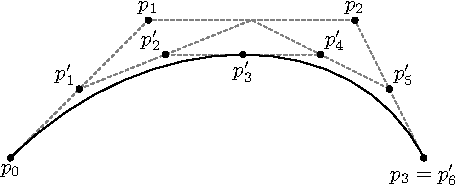
\includegraphics{subdivision}
% 	     \caption{A Figure}
% 	 \label{subd}
% 	\end{figure}
%
% \clearpage %% starts a new page and stops trying to place floats such as tables and figures
%
% \section{More Figure Stuff}
% You can also scale and rotate figures.
%  	\begin{figure}[h!]
%
% 	       \centering
% 	    % DO NOT ADD A FILENAME EXTENSION TO THE GRAPHIC FILE
% 	    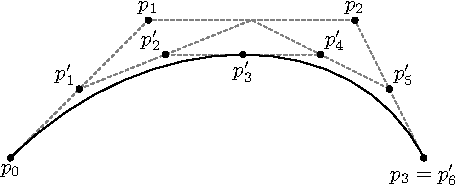
\includegraphics[scale=0.5,angle=180]{subdivision}
% 	    % if your figure shows up not where you want it, it may just be too big to fit. You can use the scale argument to shrink it, e.g. scale=0.85 is 85 percent of the original size.
% 	     \caption{A Smaller Figure, Flipped Upside Down}
% 	 \label{subd2}
% 	\end{figure}
%
% \section{Even More Figure Stuff}
% With some clever work you can crop a figure, which is handy if (for instance) your EPS or PDF is a little graphic on a whole sheet of paper. The viewport arguments are the lower-left and upper-right coordinates for the area you want to crop.
%
%  	\begin{figure}[h!]
% 	    	       \centering
% 	    % DO NOT ADD A FILENAME EXTENSION TO THE GRAPHIC FILE
% 	   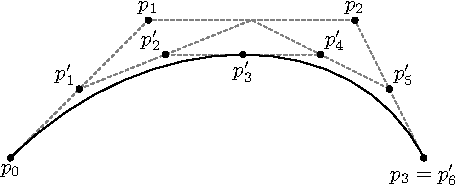
\includegraphics[clip=true, viewport=.0in .0in 1in 1in]{subdivision}
% 	    \caption{A Cropped Figure}
% 	 \label{subd3}
% 	\end{figure}
%
%       \subsection{Common Modifications}
%       The following figure features the more popular changes thesis students want to their figures. This information is also on the web at \url{web.reed.edu/cis/help/latex/graphics.html}.
%            \renewcommand{\thefigure}{0.\arabic{figure}} %Renumbers the figure to the type 0.x
%     \addtocounter{figure}{4} %starts the figure numbering at 4
%     \begin{figure}[htbp]
%     \begin{center}
%    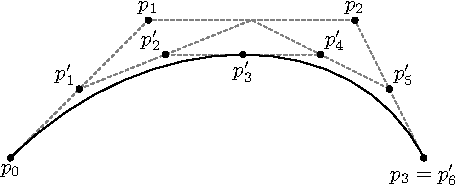
\includegraphics[scale=0.5]{subdivision}
%     \caption[Flower type and percent specialization]{\footnotesize{Interaction bar plot showing the degree of specialization for each flower type.}} %the special ToC caption is in square brackets. The \footnotesize makes the figure caption smaller
%     \label{barplot}
%     \end{center}
%     \end{figure}
%
\chapter*{Conclusion}
         \addcontentsline{toc}{chapter}{Conclusion}
	\chaptermark{Conclusion}
	\markboth{Conclusion}{Conclusion}
	\setcounter{chapter}{4}
	\setcounter{section}{0}

Here's a conclusion, demonstrating the use of all that manual incrementing and table of contents adding that has to happen if you use the starred form of the chapter command. The deal is, the chapter command in \LaTeX\ does a lot of things: it increments the chapter counter, it resets the section counter to zero, it puts the name of the chapter into the table of contents and the running headers, and probably some other stuff.

So, if you remove all that stuff because you don't like it to say ``Chapter 4: Conclusion'', then you have to manually add all the things \LaTeX\ would normally do for you. Maybe someday we'll write a new chapter macro that doesn't add ``Chapter X'' to the beginning of every chapter title.

\section{More info}
And here's some other random info: the first paragraph after a chapter title or section head \emph{shouldn't be} indented, because indents are to tell the reader that you're starting a new paragraph. Since that's obvious after a chapter or section title, proper typesetting doesn't add an indent there.


%If you feel it necessary to include an appendix, it goes here.
    \appendix
      \chapter{Algorithms \& Programs}
      \chapter{Benchmarking Graphs \& Supplemental Data}
      \chapter{Biological Data}


%This is where endnotes are supposed to go, if you have them.
%I have no idea how endnotes work with LaTeX.

  \backmatter % backmatter makes the index and bibliography appear properly in the t.o.c...

% if you're using bibtex, the next line forces every entry in the bibtex file to be included
% in your bibliography, regardless of whether or not you've cited it in the thesis.
    \nocite{*}

% Rename my bibliography to be called "Works Cited" and not "References" or ``Bibliography''
% \renewcommand{\bibname}{Works Cited}

%    \bibliographystyle{bsts/mla-good} % there are a variety of styles available;
%  \bibliographystyle{plainnat}
% replace ``plainnat'' with the style of choice. You can refer to files in the bsts or APA
% subfolder, e.g.
 \bibliographystyle{APA/apa-good}  % or
 \bibliography{thesis}
 % Comment the above two lines and uncomment the next line to use biblatex-chicago.
 %\printbibliography[heading=bibintoc]

% Finally, an index would go here... but it is also optional.
\end{document}
